\documentclass[12pt]{article}
\usepackage{graphicx}
\usepackage{amsfonts}
\usepackage{fullpage}
\begin{document}
	\tableofcontents
	\title{Belajar \LaTeX}
	\author{ilman teguh prasetya}
	\date{\today}
	\maketitle
	\section{Cara Menulis Carita Bagus}
		Berikut merupakan pembelajaran saya mengenai \LaTeX. \LaTeX merupakan sebuah markup language untuk menulis sebuah jurnal atau paper.
		
		\LaTeX  sendiri dapat membantu penulis dalam pembuatan sebuah paper, dimana papaer tersebut memerlukan penulisan rumus matematika yang sangat banyak atau complex.
		\subsection{Bangun Ruang}
		Pada Article ini saya akan mencoba untuk menulis sebuah paragraf mengenai bangun ruang. Article yang akan ditulis berisi mengenaik berbagai bangun ruang seperti persegi, segitiga dsb.
			\subsubsection{persegi}
			Persegi adalah segi empat yang sisi-sisinya sama panjang dan semua sudutnya siku - siku
			\begin{center}
						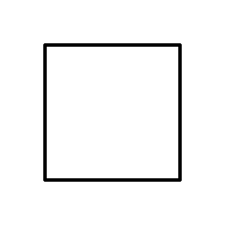
\includegraphics[width=3in]{persegi.png}
			\end{center}
			\begin{itemize}
			\item Luas 
			$$L=s \times s$$
			\begin{itemize}
			\item s = Sisi
			\end{itemize}
			\item Keliling
			$$S = 4 \times s$$
			\begin{itemize}
			\item S = Sisi
			\end{itemize}
			\end{itemize}
			\subsubsection{persegi panjang}
			Persegi Panjang adalah segi empat dengan dua pasang sisi yang saling berhadapan sejajaran dan sama panjang serta keempat sudutnya siku - siku 
			\begin{center}
						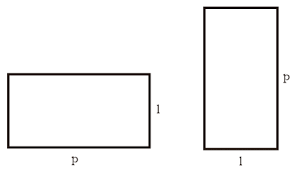
\includegraphics[width=5in]{persegi panjang.png}

			\end{center}
			\begin{itemize}
				\item Luas Persegi Panjang
				$$L=p \times l$$
				\begin{itemize}
				\item $L=luas$
				\item $keliling$
				\item $p=panjang$
				\item $l=lebar$
				\end{itemize}
				\item Keliling Persegi Panjang
				$$K=2p+2l$$
			\end{itemize}
			\subsubsection{Jajar Genjang}
			jajargenjang adalah segi empat dengan dua pasang sisi saling berhadapan sejajar dan sama panjang serta sudut-sudut yang berhadapan sama besar
			
			\begin{center}
				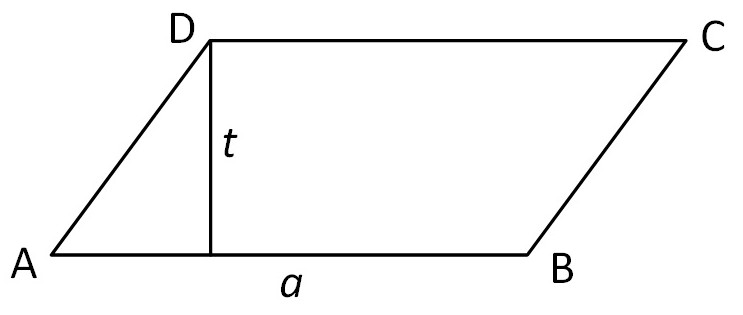
\includegraphics[width=5in]{rumus-luas-jajar-genjang.jpg}
			\end{center}
			
			
			\begin{itemize}
				\item Luas Persegi Panjang
				$$L=p \times l$$
				\begin{itemize}
				\item $L=a\times t$
				\item $keliling$
				\item $p=panjang$
				\item $l=lebar$
				\end{itemize}
				\item Keliling Persegi Panjang
				$$K=a+b+c+d$$
			\end{itemize}
			\subsubsection{Segitiga}
			Segitiga adalah bangun datar dibatasi oleh tiga sisi dan memiliki tiga sudut
			
			\begin{center}
			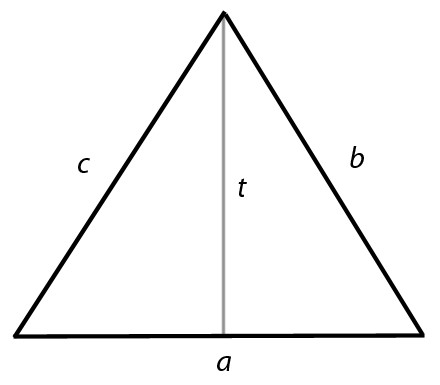
\includegraphics[width=5in]{luas-segitiga.jpg}
			\end{center}
			\begin{itemize}
			\item Luas
			$$L=\frac{1}{2} \times a \times t$$
			\item Keliling
			$$K=a+b+c$$
			\end{itemize}
			\subsubsection{Belah Ketupat}
			Belah Ketupat adalah jajargenjang yang sisi sisinya sama dan kedua diagonal saling berpotongan tegak lurus
			\begin{itemize}
			\item Luas
			$$L=\frac{1}{2} \times d_1 \times d_2 $$
			\item Keliling
			$$K=a+b+c+d$$
			\item Deskripsi
			$$L=luas$$
			$$K=keliling$$
			$$d_1=diagonal 1$$
			$$d_2=diagonal 2$$
			$$a,b,c dan d = sisi belah ketupat$$
			\end{itemize}
			\subsubsection{Trapesium}
			Trapesium adalah segi empat yang mempunyai sepasang sisi sejajar. Pada Gambar dibawah yaitu sisi $\mathbb{a}$ dengan sisi b
			\begin{itemize}
			
			\item Luas
			$$L=\frac{a+b}{2}\times t$$
			\item Keliling
			$$K=a+b+c+d$$
			\item Deskripsi
			$$L=luas$$
			$$K=keliling$$
			$$a=alas$$
			$$b=sisi yang sejajar dengan atas$$
			$$c dan d = sisi miring$$
			\end{itemize}
			\subsubsection{Layang - Layang}
			Layang-layang adalah adalah segi empay yang mempunyai dua panjang sisi sama dan mempunyai dua diagonal berpotongan tak lurus
			\subsubsection{Lingkaran}
			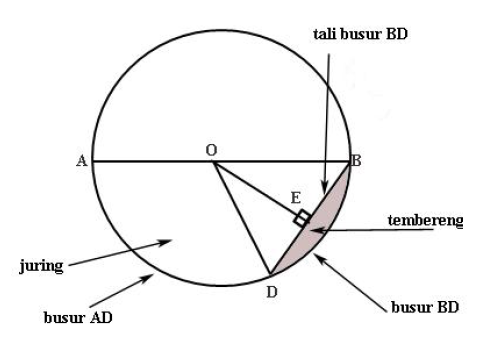
\includegraphics[width=5in]{rumus-keliling-lingkaran-dan-contoh-soalnya.png}
			\begin{itemize}
			\item Luas
			$L=\pi \times r^2$ atau $L=\pi \times \frac{1}{4} d^3$
			\item Keliling
			$K=2\times \pi \times r$
			\end{itemize}
\end{document}